
\section{Curves in Toric Surfaces}


\subsection{Introduction}

In this section, we are motivated by the following basic question: given a smooth complete curve $C$ and a toric surface $S$, when does there exists a closed immersion $C \embed S$? Likewise for the smooth complete curve $C$, we consider when there exists some toric surface $S$ with a closed immersion $C \embed S$? This question may be motivated by the toric constructure of regular normal crossings models of a curve described by \cite{tim} which requires the curve and various modifications of it to admit embeddings and smooth compactifications in specific toric surfaces. It turns out the very general answer to both questions will be negative. However, for curves which do admit such a toric embedding, we get a strong theory relating the possible toric embeddings to numerical invariants of the curve $C$ as an extension of the well-known numerical constrains on the genus of plane curves. As a first step to understanding embeddings $C \embed S$, notice there are two cases, either $C$ intersects the torus $\Gm{k}^2 \embed S$ or the image of $C$ in $S$ is contained in the toric divisor $D_{\Toric} = \bigcup C_i$ which is a union of curves which are toric varieties. In the later case, since the curve $C$ is irreducible, such an embedding gives an isomorphism between $C$ and an irreducible component of the toric divisor $C_i$ but toric varieties are clearly rational so this case can only occur when $C$ is rational. We will generally ignore this possibilitiy since $\P^1_k$ is the unique smooth complete rational curve. Therefore, we get a trivial positive answer for rational curves since $\P^1_k$ is the unique one dimensional toric variety so $\P^1_k$ can always be embedded in the toric divisor of any toric surface.
\bigskip\\
Thus, when $C$ is nonrational, any embedding $C \embed S$ into a toric surface $S$ must intersect the torus $\Gm{k}^2 \subset S$ giving a closed immersion $U \embed \Gm{k}^2$ of some open affine $U \subset C$. Therefore, our first task will be to understand closed immersions of affine curves $U \embed \Gm{k}^2$.

\begin{lemma}
Every geometrically reduced curve over $k$ is birational to some $U_f \embed \Gm{k}^2$.
\end{lemma}

\begin{proof}
Let $C$ be a curve over $k$. Then $\dim{C} = \trdeg{k}{K(C)}$ by Noetherian normalization so there is a trancendental $t \in K(C)$ such that $K(C)$ is finite over $k(t)$. If we assume that $K(C)  / k(t)$ is seperable then by the primitive element theorem $K(C) = k(t)[x]/(m(x)) = \Frac{k[t^{\pm 1}, x^{\pm 1}]/(m(x))}$ for the minimal polynomial $x$ of the primitive element. Such an isomorphism identifies open subsets of $C$ and of $\Spec{k[t, x]/(m(x))} \embed \Gm{k}^2$. 
\bigskip\\
Now, when $k(t)$ is not perfect we must be more careful to conclude that $K(C) / k(t)$ is generated by a single element. Consider $k(t) \subset E \subset K(C)$ with $E / k(t)$ the largest seperable intermediate extension then $K(C) / E$ is purely inseperable meaning that every $r \in K(C)$ satisfies $r^q \in E$ for some $q$. Choose some $r \in K(C) \setminus L$ 
(FINSIH THIS)
\end{proof}
\noindent
However, it does not suffice to take \textit{any} affine open as the following example shows, we must indeed take a sufficiently small open so the notion of birationality here is actually necessary.

\begin{prop}
There exists a smooth affine curve $C$ over $k$ with no closed immersion $C \embed \Gm{k}^2$. 
\end{prop}

\begin{proof}
We use the obstruction that any curve embedded in $\Gm{k}^2$ must have a trivial canonical bundle (Lemma \ref{plane_curve_trivial_canonical}). Therefore, it sufficees to produce a smooth affine curve with a nontrivial canonical bundle. The affiness is easy to arrange since for any smooth complete curve $\overline{C}$ then removing a single point leaves an affine curve (Lemma \ref{affine_remove_point}). Setting $C = \overline{C} \setminus \{ P \}$, the inclusion $j : C \to \overline{C}$ induces an exact sequence,
\begin{center}
\begin{tikzcd}
\Z \arrow[r] & \Cl{\overline{C}} \arrow[r, "j^*"] & \Cl{C} \arrow[r] & 0
\end{tikzcd}
\end{center}
where the first map is $1 \mapsto [P]$. Therefore, a divisor class $D$ is sent to zero under $f^* D \sim 0$ iff $D \sim \deg{D} \cdot [P]$. We need to show that the canonical divisor does not vanish $K_C \not \sim 0$ and thus that $K_{\overline{C}} \not\sim (2g - 2) \cdot [P]$ since $j : C \embed \overline{C}$ is \etale so $\Omega_{C/k} = f^* \Omega_{\overline{C}/k}$. Therefore, it suffices to produce a curve $\overline{C}$ with a point $P \in \overline{C}$ such that $K_{\overline{C}} \not\sim (2g - 2) \cdot [P]$. Note that because the $(2g - 2)$-torsion in the Picard group for $g \ge 2$ is a finite group, all but finitely many choices for $P$ on any smooth complete curve of genus $g \ge 2$ will work.
\bigskip\\
Specificially, take $\overline{C} = \Proj{k[X, Y, Z]/(X^4 - X^2 Z^2 + (Y - Z)^4 - Z^4)}$ which is easily verfified to be smooth in characteristic $p \neq 2,5$ and has genus $g = 3$ since it is a plane curve of degree $4$ in $X = \P^2_k$. Then choose $P = [0 : 0 : 1]$. Notice that under $\iota : \overline{C} \embed \P^2_k$ we have $\Omega_{\overline{C}/k} \cong \iota^* \struct{X}(1)$ by the adjunction formula. We need to check that $(2g - 2) \cdot [P]$ is not one of the effective divisors linearly equivalent to $K_{\overline{C}}$. Such divisors are parametrized by sections $H^0(\overline{C}, \Omega_{\overline{C}/k}) = H^0(X, \iota_* \iota^* \struct{X}(1))$. By the projection formula $\iota_* \iota^* \struct{X}(1) = \iota_* \struct{\overline{C}} \otimes_{\struct{X}} \struct{X}(1)$. To compute the sections of this coherent $\struct{X}$-module we apply the exact sequence of the Cartier divisor $\overline{C}$ twisted by $\struct{X}(1)$,
\begin{center}
\begin{tikzcd}
0 \arrow[r] & \struct{X}(-3) \arrow[r] & \struct{X}(1) \arrow[r] & \iota_* \struct{\overline{C}} \otimes_{\struct{X}} \struct{X}(1) \arrow[r] & 0
\end{tikzcd}
\end{center}
and applying cohomology,
\begin{center}
\begin{tikzcd}
H^0(X, \struct{X}(-3)) \arrow[r] & H^0(X, \struct{X}(1)) \arrow[r] & H^0(\overline{C}, \iota^* \struct{X}(1)) \arrow[r] &  H^1(X, \struct{X}(-3)) 
\end{tikzcd}
\end{center}
but $H^q(X, \struct{X}(-3)) = 0$ for $q \le 1$ so the map $H^0(X, \struct{X}(1)) \onto H^0(\overline{C}, \iota^* \struct{X}(1))$ given by pulling back sections, $s \mapsto \iota^* s$, is bijective. In particular, since any section $s \in H^0(\overline{C}, \Omega_{\overline{C}/k})$ is the pullback of some hyperplane equation $h \in H^0(X, \struct{X}(1))$, the divisor of zeros associated to $s$ is the hyperplane section $\iota^{-1}(H) = \overline{C} \cap H$ with the hyperplane $H = V(h)$. However, I claim that any line passing through $P$ intersects $\overline{C}$ in more than one point. To see this, consider the tangent line $L$ to $\overline{C}$ at $P$ is $\P^1_k \to X$ given by $[T_0 : T_1] \mapsto [T_0 : 0 : T_1]$ but $L \cap \overline{C} = \{[0 : 0 : 1], [1 : 0 : 1], [-1 : 0 : 1] \}$. Therefore, there cannot be any line passing through only $P$ meaning that $\{ P \}$ cannot be the support of any effective divisor in canonical linear system $H^0(\overline{C}, \Omega_{\overline{C}/k})$. Thus, $K_{\overline{C}} \not\sim (2g - 2) \cdot [P]$ so $C = \overline{C} \setminus \{ P \}$ has nontrivial canonical bundle yet is affine providing the required example.
\end{proof}

\begin{rmk}
Notice that although $C$ is not an affine plane curve (in the sense of having a closed immersion $C \embed D(q) \subset \A^2_k$ to some principal affine open) there is an immersion $C \embed \P^2_k$ since $\overline{C} \embed \P^2_k$ is a complete plane curve.
\end{rmk}
\noindent
We conclude by providing proofs of the required lemmas.

\begin{lemma} \label{plane_curve_trivial_canonical}
Let $C \embed D(q) \subset \A^2_k$ be a smooth curve embedded in some standard open $D(q)$ in the affine plane. Then the canoncial bundle $\Omega^1_{C/k} \cong \struct{C}$ is trivial.
\end{lemma}

\begin{proof}
Let $A = k[x, y, q^{-1}]$ so $D(q) = \Spec{A}$. Note that $C = \Spec{R}$ with $R = A/I$ where $I = \ker{(A \to \Gamma(C, \struct{C}))}$. Furthermore, $I = (f)$ since $\dim{C} = 1$ thus $\height{I} = 1$ but $C$ is irreducible and thus $I$ is prime and since $A$ is a UFD, $I = (f)$ since each height one prime is principal. Furthermore, $C$ is smooth so $(f, f_x, f_y) = A$ where $f_x, f_y$ are the partial derivatives of $f$ with respect to $x$ and $y$. Therefore, we can choose $g,h \in A$ such that $g f_x + h f_y = 1$ in $R$. Now, consider the $R$-module of differentials, $\Omega_{R/k} = (R \d{x} \oplus R \d{y}) /(f_x \d{x} + f_y \d{y})$. 
\bigskip\\
Consider the map $\phi : R \to \Omega_{R/l}$ sending $1 \mapsto h \d{x} - g \d{y}$. Note that,
\[ \d{x} = g f_x \d{x} + h f_y \d{x} = h f_y \d{x} - g f_y \d{y} \implies f_y \mapsto \d{x} \] 
\[ d{y} = g f_x \d{y} + h f_y \d{y} = g f_x \d{y} - h f_x \d{x} \implies -f_x \mapsto \d{y} \]
so $\phi$ is surjective. Furthermore, suppose that $\phi(a) = 0$ then $\phi(f_x a) = \phi(f_y a) = 0$ so in $R \d{x} \oplus R \d{y}$ we have $a \d{x}, a \d{y} \in (f_x \d{x} + f_y \d{y})$  meaning $a \d{x} = c_1(f_x \d{x} + f_y \d{y})$ and $a \d{y} = c_2(f_x \d{x} + f_y \d{y})$ giving $c_1 f_y = 0$ and $c_2 f_x = 0$ and $c_1 f_x = c_2 f_y = a$ since $R \d{x} \oplus R \d{y}$ is free. But then \[ a = g f_x a + h f_y a = g f_x c_2 f_y + h f_y c_1 f_x = 0 \]
since $c_2 f_x = c_1 f_y = 0$ so $\phi$ is injective. Thus $\Omega_{R/k} \cong R$ and sheafifying gives, $\Omega_{C/k} \cong \struct{C}$. 
\end{proof}

\begin{lemma} \label{affine_remove_point}
Let $C$ be a smooth proper curve and $P \in C$ a point. Then $C \setminus \{ P \}$ is affine. 
\end{lemma}

\begin{proof}
The divisor $D = \nu [P]$ is very ample for sufficiently large $\nu$ (in fact for $\nu \ge 2 g + 1$) [Har, IV.3.2]. Therefore, the linear system $|\nu [P]|$ defines a closed ($C$ is proper) immersion $j : C \embed \P^{\nu - 1}_k$ such that $\struct{C}(D) = j^* \struct{\P^{\nu-1}_k}(1)$ with the hyperplane sections pulling back to a basis of $H^0(C, \struct{C}(D))$. Since $D$ is effective, there is some section $s \in H^0(C, \struct{C}(D))$ with $V(s) = \{ P \}$ and thus some hyperplane section $h \in H^0(\P^{\nu - 1}_k, \struct{\P^{\nu-1}_k}(1))$ with $s = j^* h$ and thus $\{ P \} = j^{-1}(H \cap j(C))$ where $H = V(h) \subset \P^{\nu - 1}_k$. Finally, $C  \setminus \{ P \} = j^{-1}(\P^{\nu - 1}_k \setminus H)$ which is affine since $j$ is a closed immersion and thus affine and the complement of a hyperplane in projective space is a standard open.
\end{proof}


\subsection{Polytopes and Laurent Polynomials}

In order to understand the moduli of curves which lie in toric surfaces, we would like to understand and develop a dictionary relating combinatorial features of defining data of a curve inside the torus to geometric properties of the complete curve inside the toric completion. This dicussion relies upon the easy fact that curves inside the torus are defined uniquely up to unimodular transformation by Laurent polynomials which are objects well suited to description by combinatorial data.

\begin{prop}
Curves $C_0 \subset \Gm{k}^2$ are exactly $V(f)$ for some Laurent polynomial $f \in k[x^{\pm 1}, y^{\pm 1}]$ unique up to automorphism of the torus.
\end{prop}

\begin{proof}
A closed immersion $C_0 \embed \Gm{k}^2$ is codimension $1$ and thus is defined by some ideal $I \subset R = k[x^{\pm 1}, y^{\pm 1}]$ of height $1$. Since $C_0$ is reduced we may take $I$ to be racial and thus it is the intersection of the minimal primes $\p$ over $I$ which have height one as well. Since $R/I$ is noetherian there are finitely many such minimal primes over $I$. Finally, since $R$ is a UFD height one primes are principal and thus $I = \bigcap \p_i = \bigcap (p_i) = (p_1 \cdots p_r)$ is principal and determined up to a unit in $R$ corresponding to an automorphism of $\Gm{k}^2$.
\end{proof}
\noindent
Given an irreducible Laruent polynomial $f \in k[x^{\pm 1}, y^{\pm 1}]$ we denote the associated curve in the torus $V(f) \subset \Gm{k}^2$ by $U(f)$ following the notation of [CASTRYCK]. 

\begin{rmk}
Recall that the automorphism group of the $n$-torus $\Aut{\Gm{k}^n}$ is exactly $k^\times \times \GL{n}{\Z}$ with the following action on coordinate ring $k[x_1^{\pm 1}, \dots, x_n^{\pm 1}]$,
\begin{equation}
(r,  A) \cdot x_j = r \prod_{i = 1}^n x_i^{a_{ij}} \quad \text{ where } \quad r \in k^\times \quad \text{ and } \quad A = (a_{ij}) \in \GL{n}{\Z} 
\end{equation}
Note that if we restrict to automorphism of the torus \text{as a group scheme} then $\Aut{\Gm{k}^n} = \GL{n}{\Z}$ setting $r = 1$ and thus preserving the identity. 
\end{rmk}

\noindent
The most important combinatorial data which can be extracted from a Laurent polynomial is its Newton polygon.


\begin{defn}
Given a Laurent polynomial $f \in k[x^{\pm 1}, y^{\pm 1}]$, its Newton polygon $\Delta(f) \subset \R^2$ is the following convex polygon,
\begin{equation}
\Delta(f) = \mathrm{Conv} \left( \{ (i,j) \mid a_{ij} \neq 0 \} \right) \quad \text{ where } \quad f = \sum_{i,j} a_{ij} x^i y^i 
\end{equation}
\end{defn}

\begin{defn}
For a convex rational polygon $\Delta$ we define,
\[ \Delta^{(1)} = \Conv{\Delta^\circ \cap \Z^2} \]
when $\Delta$ is a lattice polygon then $\Delta^{(1)}$ corresponds to shifting the faces of $\Delta$ inwards by one unit. Furthermore, if $\Gamma$ is a polygon then let $\Gamma^{(-1)}$ be the \textit{outward} shift by one unit (note $\Gamma^{(-1)}$ is a lattice polygon iff $\Gamma = \Delta^{(1)}$ for some lattice polygon $\Delta$). Then we define $\Delta^{\text{max}} = \Delta^{(1)(-1)}$.
\end{defn}

\noindent
We will begin our discussion of the combinatorial dictionary with the most fundamental question, when the complete curve inside the toric completion is smooth. 

\begin{defn}
We say that $f \in k[x^{\pm 1}, y^{\pm 1}]$ is \textit{nondegenerate with respect to its Newton polygon} if for each face $\tau \subset \Delta(f)$ (including $\Delta(f)$ itself then the Laurent polynomials,
\[ f|_\tau, \partial_x f|_\tau, \partial_y f|_\tau \]
generate the unit ideal where we define restriction to a face $f|_\tau$ via the formula,
\[ f |_{\tau} = \sum_{(i, j) \in \tau} a_{ij} x^i y^i \quad \text{ where } \quad f = \sum_{(i,j) \in \Delta(f)} a_{ij} x^i y^j \]
For a fixed convex lattice polytope $\Delta \subset \R^2$ we say that $f$ is $\Delta$-nondegenerate if $\Delta(f) = \Delta$ and $f$ is non-degenerate with respect to its Newton polygon. 
\end{defn}
\noindent
This definition will be important in the context of the following construction which, given a Laurent polynomial $f$, constructs a smooth complete curve living on a toric surface birational  to $U_f$ via toric completion. However, some nondegeneracy condition on the defining Laurent polynomial will be necessary to ensure that the resulting complete curve is indeed smooth. We shall see that $\Delta$-nondegeneracy will suffice. Abstractly, the construction goes as follows. Given a Laurent polynomial $f \in k[x^{\pm 1}, y^{\pm 1}]$ defining a curve $C_0 = U_f \subset \Gm{k}^2$ and a convex lattice polytope $\Delta$, consider the locally closed immersion $C_0 \embed \Gm{k}^2 \embed \Toric_\Delta$ and let $C_0^\Delta$ be the scheme-theoretic image. Then clearly, $C_0^\Delta$ is a projective (and thus complete) curve on $\Toric_\Delta$ but it remains to see when $C_0^\Delta$ is smooth. We can describe this construction in a somewhat more geometrically satisfying way by considering the explicit projective embedding of the toric surface $\Toric_\Delta$ defined as follows. Let $N = | \Delta \cap \Z^2| - 1$ and consider the monomials $s_p = x^i y^j$ where $p = 0, 1, \dots, N$ indexes the lattice points $p(i, j) \in \Delta \cap \Z^2$. We consider these monomials as sections $s_p \in \Gamma(\Gm{k}^2, \struct{\Gm{k}^2})$ which trivially generate the structure sheaf and thus define a morphism $\Gm{k}^2 \embed \P^N$ which it is straightforward to verify is a locally closed immersion. Then $\Toric_\Delta$ is the scheme-theoretic image inside $\P^N$. Explicitly, the immersion $\psi : \Toric_\Delta \embed \P^N$ is given by the linear system $|D_\Delta|$ for the divisor associated to the polytope $\Delta$ since these sections $x^i y^j$ for $(i, j) \in \Delta$ are exactly the characters $x^i y^j \in H^0(\Toric_\Delta, \struct{\Toric_\Delta}(D_\Delta))$. As we have seen (Proposition \ref{polytope_div_ample}), the divisor $D_\Delta$ associated to $\Delta$ is strictly convex and thus ample (and globally generated) but for $n = \dim{\Toric_\Delta} = 2$ then $D_\Delta$ is very ample so $\Toric_\Delta \embed \P^N$ is an immersion and $\struct{\Toric_\Delta}(D_\Delta) = \psi^* \struct{\P^N}(1)$. 
This map is always a closed embedding for proper toric surfaces, in general replacing a polygon $P$ by $(n-1)P$ will make the immersion defined by the linear system $|D_P|$ into a closed immersion (Theorem \ref{divisor_positivity} (c)). The curve $C^\Delta_0$ is then a hyperplane section of $\Toric_\Delta \subset \P^N$ defined by the hyperplane,
\[ H_C = \sum_{(i, j) \in \Delta(f)} a_{ij} X_{ij} \quad \text{ where } \quad f = \sum_{(i,j) \in \Delta(f)} a_{ij} x^i y^j \]
where $\P^N$ is given coordinates $X_{ij}$ for each $(i,j) \in \Delta$ and the map $\Gm{k}^2$ may be described via the formula, $(x,y) \mapsto (X_{ij} = x^i y^j)$. Then it is clear that the vanishing of $f$ extended to $\Toric_\Delta$ corresponds to the intersection of $\Toric_\Delta$ and the above hyperplane.  
\bigskip\\
We can now give a geometric interpretation of the $\Delta$-nondegenerate condition from the following proposition.

\begin{prop}
A Laurent polynomial $f \in k[x^{\pm 1}, y^{\pm 1}]$ defining a torus curve $C_0 = U_f$ is $\Delta$-nondegenerate exactly when for each face $\tau \subset \Delta$, the intersection of the complete curve $C^\Delta_0$ and the torus orbit $V(\tau)$ is smooth and of codimension $1$ i.e. $\codim{C^\Delta_0 \cap V(\tau), V(\tau)} = 1$ and $C^\Delta_0 \cap V(\tau)$ is smooth.
\end{prop}

\begin{proof}
A full proof can be found in Batyrev [3, Section 4], here we give a sketch.  (DOOO THISS!!!)
\end{proof}
\noindent
Note that this condition tells us about the nature of the intersection of the curve $C^\Delta_0$ and $\Toric_\Delta \setminus \Toric^2$. In particular, they must intersect transversally in order that the intersection be smooth and of codimension. Furthermore, the vertices of $\Delta$ correspond to dimension zero orbits (which are the intersection of the irreducible components of $\Toric_\Delta \setminus \Toric^2$) and thus their intersection with $C^\Delta_0$ must be empty. Furthermore, since $\Toric_\Delta$ is always normal, smoothness in codimension one implies that the discussed intersection conditions are equivalent to those in the conclusion of the lemma. In summary, $\Delta$-nondegenerate equations are those which define smooth curves in $\Toric_\Delta$ which intersects the toric boundary transversally and outside its intersection points.

(INSERT IMAGE)

This condition on the nature of the intersection with the toric boundary is less intrisic to the curve (for examle, fixing a $\Gm{k}^2 \subset \P^2_k$ and a plane curve $C \subset \P^2_k$ we can always move the curve such that it intersects the three lines of the compliment of the torus transversally and does not pass through the intersection points of these three lines) and will often be inconsequental for results we would like to prove about such objects. Thus we define the weaker notion which ignores this intersection criterion.

\begin{defn}
We say that a Laurent polynomial $f \in k[x^{\pm 1}, y^{\pm 1}]$ is $\Delta$-toric if $f$ defines a smooth curve $C_0 = U_f$ whose $\Delta$-toric completion $C^\Delta_0 \embed \Toric_\Delta$ is smooth.
\end{defn}
\noindent
In the next section we will see how to reinterpret this condition purely in terms of properties of $f$, its Newton polygon, and the affine curve $U_f$.


\subsection{Baker's Theorem on the Genus for Toric Embeddings}

In this section, we discuss the classical result of Baker (1893) relating the genus of a smooth curve compactified in a toric surface to the enumerative properties of its associated convex lattice polygon. We also discuss a further result which relates another important algebrogeometric invariant of the curve, its gonality, to the numerical properties of the Newton polygon.

\begin{thm}[Baker]
Let $f \in k[x^{\pm 1}, y^{\pm 1}]$ be a $\Delta$-nondegenerate Laurent polynomial. Then the toric completion $C_0^\Delta \embed \Toric_\Delta$ of $C_0 = U_f$ is a smooth Cartier divisor on $\Toric_\Delta$ and thus $C_0^\Delta$ is the unique smooth proper curve birational to $C_0$. Furthermore, the genus is computed via the number of interior lattice points of the Newton polygon, 
\[ g(C_0^\Delta) = |\Delta^\circ \cap \Z^2| \]
\end{thm}

\begin{proof}
Since $f$ is $\Delta$-nondegenerate, then $C_0^\Delta$ is an integral codimension one closed subscheme which does not intersect the singular locus of $\Toric_\Delta$ (in particular for $x \in C_0^\Delta$ then $\stalk{\Toric_\Delta}{x}$ is a UFD) so $C_0^\Delta$ is Cartier. Let $C = C_0^\Delta$ then to compute the genus of $C$ we need to understand the space of sections of its canonical sheaf $\omega_C$. Fixing notation, let $X = \Toric_\Delta$ and let $\iota : C \embed X$ be the inclusion. Choose a torus-invariant Cartier divisor $D_C$ linearly equivalent to the effective Cartier divisor $C$, in fact, we can explicilty write $D_C = C - \div{(f)}$ which is torus-invariant because it is supported on the toric divisor since $C|_{\Toric^n} = \div{(f)}|_{\Toric^n}$. We will now apply the adjunction exact sequence defined in Theorem \ref{adjunction},
\begin{center}
\begin{tikzcd}
0 \arrow[r] & \omega_X \arrow[r, "f"] & \omega_X(D_C) \arrow[r] & \iota_* \omega_C \arrow[r] & 0
\end{tikzcd}
\end{center}
where the dualizing sheaf $\omega_C$ is, because $C$ is smooth, is the canonical bundle. The cohomology long exact sequnce gives,
\begin{center}
\begin{tikzcd}
0 \arrow[r] & H^0(X, \omega_X) \arrow[r] & H^0(X, \struct{X}(D_C + K_X)) \arrow[r] & H^0(C, \omega_C) \arrow[r] & H^1(X, \omega_X)
\end{tikzcd}
\end{center} 
But $H^0(X, \omega_X) = H^0(X, \struct{X}(K_X)) = 0$ since the canonical divisor    has an empty corresponding polytope $P_{K_X} = \varnothing$. Furthermore, $H^1(X, \omega_X) = H^0(X, \struct{X}) = 0$ by Serre duality and Demazure vanishing. Therefore, the cohomology sequence gives an isomorphism,
\[ H^0(X, \struct{X}(D_C + K_X)) \xrightarrow{\sim} H^0(C, \omega_C) \]
In particular, the genus is,
\[ g(C) = \dim_k H^0(X, \struct{X}(D_C + K_X)) = | P_{D_C + K_X} \cap \Z^2 | \]
Thus, we need to compute $P_{D_C}$. Recall that under the embedding $\psi : \Toric_\Delta \embed \P^N_k$ the curve $C$ is the hyperplane section defined by the hyperplane,
\[ H_C = \sum_{(i, j) \in \Delta} a_{ij} X_{ij} \quad \text{ where } \quad f = \sum_{(i,j) \in \Delta} a_{ij} x^i y^j \]
Therefore, $\struct{X}(C) = \psi^* \struct{\P^N}(H_C) \cong \psi^* \struct{\P^N}(1)$ but recall that $\struct{X}(D_\Delta) = \psi^* \struct{\P^N}(1)$ so we find that $\struct{X}(C) \cong \struct{X}(D_\Delta)$. Therefore, $D_C \sim C \sim D_\Delta$ but both $D_C$ and $D_\Delta$ are torus-invariant so $P_{D_C} \cong_t \Delta$ (using that $P_{D_\Delta} = \Delta$). Decomposing,
\[ \Delta = \bigcap_{\substack{F \subset \Delta \\ \text{facet}}} H^+(n_F, - a_F) \]
we find,
\[ D_C \sim \sum_{\substack{F \subset \Delta \\ \text{facet}}} a_F D_F \]
Recall the canonical divisor is,
\[ K_X = - \sum_{\substack{F \subset \Delta \\ \text{facet}}} D_F \]
Thus,
\[ D_C + K_X \sim \sum_{\substack{F \subset \Delta \\ \text{facet}}} (a_F - 1) D_F \]
which implies that,
\[ P_{D_C + K_X} \cong_t \bigcap_{\substack{F \subset \Delta \\ \text{facet}}} H^+(n_F, 1 - a_F) = \Delta^{(1)} \]
since $\Delta$ is a lattice polygon. Therefore, we conclude,
\[ g(C) = | \Delta^{(1)} \cap \Z^2 | = | \Delta^\circ \cap \Z^2 | \]
\end{proof}

(RELATE THIS ABOVE FACT TO CANONICAL EMBED)

\begin{theorem} \label{adjunction}
Let $X$ be a normal projective Cohen-Macaulay variety, and $\iota : C \embed X$ a divisor, and $D_C = C - \div{(f)}$ a linearly equivalent Weil divisor. Then there is an exact sequence,
\begin{center}
\begin{tikzcd}
0 \arrow[r] & \omega_X \arrow[r, "f"] & \omega_X(D_C) \arrow[r] & \iota_* \omega_C \arrow[r] & 0
\end{tikzcd}
\end{center}
\end{theorem}

\begin{proof}
The sheaf $\struct{X}(-D_C)$ is isomorphic to the sheaf of ideals defining $\iota : C \embed X$ giving an exact sequence,
\begin{center}
\begin{tikzcd}
0 \arrow[r] & \struct{X}(-D_C) \arrow[r, "f"] & \struct{X} \arrow[r] & \iota_* \struct{C} \arrow[r] & 0
\end{tikzcd}
\end{center}
Note that when $C \embed X$ is an effective Cartier divisor then $\struct{X}(-D_C)$ is its defining invertible sheaf of ideals.
Applying the functor $\shHom{\struct{X}}{-}{\omega_X}$ to the above short exact sequence gives a long exact sequence,
\begin{center}
\begin{tikzcd}
0 \arrow[r] & \shHom{\struct{X}}{\iota_* \struct{C}}{\omega_X} \arrow[r] \arrow[draw=none]{d}[name=Z, shape=coordinate]{} & \shHom{\struct{X}}{\struct{X}}{\omega_X} \arrow[r, "f"] & \shHom{\struct{X}}{\struct{X}(-D_C)}{\omega_X} 
\arrow[dll,
rounded corners, crossing over,
to path={ -- ([xshift=2ex]\tikztostart.east)
|- (Z) [near end]\tikztonodes
-| ([xshift=-2ex]\tikztotarget.west)
-- (\tikztotarget)}]
\\
& \shExt{1}{\struct{X}}{\iota_* \struct{C}}{\omega_X} \arrow[r] & \shExt{1}{\struct{X}}{\struct{X}}{\omega_X} \arrow[r] & \cdots
\end{tikzcd}
\end{center}
Since $\shHom{\struct{X}}{\struct{X}}{-}$ is the identity functor, we get $\shExt{1}{\struct{X}}{\struct{X}}{-} = 0$. Furthermore, by duality, $\shHom{\struct{X}}{\iota_* \struct{C}}{\omega_X}) = 0$ since top cohomology of $\iota_* \struct{C}$ vanishes because $\iota$ is affine and $\struct{C}$ has vanishing cohomology above degree one. Therefore, we find an exact sequence,
\begin{center}
\begin{tikzcd}
0 \arrow[r] & \omega_X \arrow[r, "f"] & \shHom{\struct{X}}{\struct{X}(-D_C)}{\omega_X} \arrow[r] & \shExt{1}{\struct{X}}{\iota_* \struct{C}}{\omega_X} \arrow[r] & 0
\end{tikzcd}
\end{center}
However, $X$ is Cohen-Macaulay and $C$ is in codimension one so $\shExt{1}{\struct{X}}{\iota_* \struct{C}}{\omega_X}$ computes the dualizing sheaf $\iota_* \omega_C$ [CITE THIS IN STACKS PROJECT].

If $C$ is Cartier, then $\struct{X}(-D_C)$ is invertible so,
\[ \shHom{\struct{X}}{\struct{X}(-D_C)}{\omega_X} = \struct{X}(D_C) \otimes_{\struct{X}} \omega_X = \omega_X(D_C) = \struct{X}(D_C + K_X) \]
To show this in the non Cartier case, we need to make a diversion into reflexive sheaves. When $X$ is a normal projective variety, the dualizing sheaf is reflexive giving a canonical divisor $\omega_X = \struct{X}(K_X)$. Furthermore, the following formula holds for reflexive sheaves on normal varieties (CITE THIS),
\[ \shHom{\struct{X}}{\struct{X}(-D)}{\struct{X}(E)} = \struct{X}(D + E) \]
Thus, we do get an exact sequence,
\begin{center}
\begin{tikzcd}
0 \arrow[r] & \struct{X}(K_X) \arrow[r, "f"] & \struct{X}(D_C + K_C) \arrow[r] & \iota_* \omega_C \arrow[r] & 0
\end{tikzcd}
\end{center}
viewing $f$ as a section of $\struct{X}(D_C)$, using that $D_C + \div{(f)} = C$ is effective, gives $\struct{X} \xrightarrow{f} \struct{X}(D_C)$. Then, tensoring by $- \otimes_{\struct{X}} \omega_X$ and using $\struct{X}(D) \otimes_{\struct{X}} \struct{X}(E) \to \struct{X}(D + E)$ via $f \otimes g \mapsto fg$ gives the above map.
\end{proof}

\noindent
The previous theorem shows that $\Delta$-nondegeneracy is sufficient for the closure of $U_f$ to embed smoothly. However, it is not necessary since the condition requires that the curve does not pass through the codimension-two toric components. We will use the following remark to weaken our nondegeneracy condition on $f$. First, we prove an extension of Baker's theorem which applies without the nondegeneracy condition.

\begin{thm} \label{baker_refinement}
For \textit{any} Laurent polynomial $f \in k[x^{\pm 1}, y^{\pm 1}]$ such that $U_f$ is a curve and $\Delta(f) = \Delta$,
\[ g(U_f) \le | \Delta^\circ \cap \Z^2 | \]
with equality exactly when the scheme theoretic image of $U_f \embed \Toric_\Delta$ is smooth. 
\end{thm}

\begin{proof}
(See [Computing zeta functions of nondegenerate curves (2007)]) We give a sketch of the proof. Let $N = | \Delta \cap \Z^2 |$ and $V$ be the number of vertices of $\Delta$ then the parameter space of Laurent polynomials $f \in k[x^{\pm 1}, y^{\pm 1}]$ such that $\Delta(f) = \Delta$ is exactly $L = \A_k^{N-V} \times_k \Gm{k}^V$ where we associate a $k$-rational point $(a_{ij}) \in \A_k^{N-V} \times_k \Gm{k}^V$ to the Laurent polynomial,
\[ f = \sum_{(i,j) \in \Delta} a_{ij} x^i y^j \]
Note that $\Delta(f) = \Delta$ since the coefficients $a_{ij}$ corresponding to vertices $(i,j) \in \Delta$ are nonzero.
Now, consider the closed subscheme,
\[ V \subset \Gm{k}^2 \times_k \A_k^{N - V} \times_k \Gm{k}^V = \Spec{k[x^{\pm 1}, y^{\pm 1}]} \times \Spec{k[a_{ij}, a_{i,j}^{-1} |_{(i,j) \in V}]} \]
defined by the vanishing,
\[ V = V\left( \sum_{(i,j) \in \Delta} a_{ij} x^i y^j \right) \]
Then the projection gives a family $\pi : V \to L$ of torus curves parametrized by the coefficients of their Laurent polynomials. Now, we complete $V$ under the open immersion $\Gm{k}^2 \times_k L \embed \Toric_\Delta \times_k L$ to get a closed immersion $\C \embed \Toric_\Delta \times_k L$ whose fiber over $f$ gives the $\Delta$-toric completion of $U_f$, 
\begin{center}
\begin{tikzcd}[row sep = huge]
V \arrow[r, hook] \arrow[drr] & \C \arrow[r, hook] \arrow[dr] & \Toric_\Delta \times_k L \arrow[d, "\pi"]
\\
& & L
\end{tikzcd}
\end{center}
By [Computing zeta functions of nondegenerate curves (2007) Section 2 Proposition 1], the locus of $L$ corresponding to $\Delta$-nondegenerate $f$ contains a Zariski dense open. Therefore, the general fiber $\mathcal{C}_{f_0}$ above $f_0 \in k[x^{\pm 1}, y^{\pm 1}]$ corresponds to $C_0^\Delta$, the completion of $C_0 = U_{f_0}$, which is smooth proper curve with genus and thus arithmetic genus,
\[ g_a(U_f^\Delta) = g(U_f^\Delta) = | \Delta^\circ \cap \Z^2 | \]
by the version of Baker's theorem proven above. I claim the family $\C \to L$ is flat. First, the projection $X = \Toric_{\Delta} \times_k L \to L$ is flat and consider $\stalk{L}{\pi(x)} \to \stalk{X}{x}$ then we take the germ $f \in \stalk{X}{x}$ when $x \in \Gm{k}^2 \times_k L$ given by,
\[ f = \sum_{(i,j) \in \Delta} a_{ij} x^i y^j \]
Then $f \in \stalk{X}{x} / \m_{\pi{x}} \stalk{X}{x} = \stalk{X}{x}\otimes_{\stalk{L}{\pi(x)}} \kappa(\pi(x))$ is a zero divisor exacly when not all $a_{ij} \in \m_{\pi(x)}$ since $x,y$ are invertible on $\Gm{k}^2$. However, since the Newton polygon is held fixed on $L$ we never have the vanishing of all $a_{ij}$. Then applying [Tag 046Z] we see that $\stalk{L}{\pi(x)} \to \stalk{X}{x}/(f)$ is flat and thus $\C \to L$ is flat. (THIS IS NOT QUITE RIGHT) Furthermore, $\C \embed \Toric_\Delta \times_k L\embed \P^n_k \times_k L$ is a closed subscheme which implies [Hartshorne III 9.10] that the arithmetic genus of the fibers is constant. Thus, for any $f \in k[x^{\pm 1}, y^{\pm 1}]$ such that $U_f$ is a smooth curve, then its toric completion $U_f^\Delta$ has arithmetic genus,
\[ g_a(U_f^\Delta) = g_a(C_0^\Delta) = | \Delta^\circ \cap \Z^2 | \]
We use the following lemmas to conclude that,
\[ g(U_f) = g(U_f^\Delta) \le g_a(U_f^\Delta) = | \Delta^\circ \cap \Z^2 | \]
which equality exactly when $U_f^\Delta$ is smooth. Furthermore, since $\C \to L$ is a proper flat family, by Zariski connectedness the fibers are connected so we see that \textit{any} $U_f^\Delta$ with $\Delta(f) = \Delta$ is connected (even when $U_f$ is not a curve i.e. not connected).
\end{proof}

\begin{rmk}
We have shown that $U_f^\Delta$ is connected whenever $\Delta(f) = \Delta$ but the affine curve $U_f$ certainly may not be. For example, consider $f_1 = (x + y - 1)(x + y + 1)$ and $f_2 = x^2 + y^2 - 1$ then $\Delta(f_1) = \Delta(f_2) = 2 \Sigma$ where $\Sigma$ is the unit isosceles right triangle. However, 
\[ U_{f_1} = \Spec{k[x^{\pm 1}, y^{\pm 1}]/(f_1)} = \Spec{k[k[x^{\pm 1}, y^{\pm 1}]/(x + y - 1)} \times_k \Spec{k[k[x^{\pm 1}, y^{\pm 1}]/(x + y + 1)} \]
which is the union of two parallel lines in $\Gm{k}^2$ (which do not intersect in the torus) while,
\[ U_{f_2} = \Spec{k[x^{\pm 1}, y^{\pm 1}]/(f_2)} = \Spec{k[x^{\pm 1}, y^{\pm 1}]/(x^2 + y^2 - 1)} \]
is irreducible and thus connected. However, in the toric completion $U_{f_1}^\Delta$ (which lies in $\Toric_{2 \Sigma} = \P^2_k$), these two parallel lines do infact intersect so both $U_{f_1}^\Delta$ and $U_{f_2}^\Delta$ are connected.
\end{rmk}


\begin{defn}
We say that $f \in k[x^{\pm 1}, y^{\pm 1}]$ is \textit{weakly} $\Delta$-\textit{nondegenerate} when the following hold,
\begin{enumerate}
\item $\Delta(f) \subset \Delta$
\item for each face $\tau \subset \Delta$ we have $\tau \cap \Delta(f) \neq \empty$
\item the affine curve $U_f$ is smooth with genus $g(U_f) = | \Delta^{(1)} \cap \Z^2 |$. 
\end{enumerate}
\end{defn}
\noindent
Weakly $\Delta$-nondegenerate Laurent polynomials $f \in k[x^{\pm 1}, y^{\pm 1}]$ do indeed define affine curves $U_f$ with an embedding $U_f \embed \Toric_\Delta$ such that the completion $C_0^\Delta$ is smooth and satisfies the numerical genus condition of Baker. However, such curves will not, in general, be Cartier divisors on $\Toric_\Delta$ since they may pass through the singular locus where $\Toric_\Sigma$ is not locally factorial. 

\begin{lemma}
In the third condition definition of weakly $\Delta$-nondegenerate Laurent polynomials, it is equivalent to assume that the scheme theoretic image of $U_f \embed \Toric_\Delta$ is smooth. 
\end{lemma}

\begin{proof}
When $U_f^\Delta$ is smooth then we have $g(U_f^\Delta) = g_a(U_f^\Delta) = | \Delta^\circ \cap \Z^2|$. Conversely, we have that $\tilde{\Delta} = \Delta(f) \subset \Delta$ (from the definition that $f$ is weakly $\Delta$-nondegenerate) and we assume $g(U_f) = | \Delta^\circ \cap \Z^2 |$. From Baker's bound,
\[ g(U_f^\Delta) = g(U_f) \le |\tilde{\Delta}^\circ \cap \Z^2| \le |\tilde{\Delta}^\circ \cap \Z^2 | \] 
Thus, from the assumption these are equalities so,
\[ g(U_f^\Delta) = | \tilde{\Delta}^\circ \cap \Z^2 | \]
and thus $U_f^\Delta$ is smooth by the above result.
\end{proof}

\subsection{Work In Progress}

\begin{defn}

\end{defn}

LATER WE NEED TO DO THIS

Furthermore, there is bijection of $\Gal{k^{\sep}/ k}$-sets,
\[ C_0^\Delta(\bar{k}) \setminus C_0^\Delta \cong \coprod_{\tau \subset \partial \Delta}  \]

\subsection{Combinatorial Gonality (WIP)}

\begin{defn}
Let $C$ be a curve over $k$. The \textit{gonality} $\gon{C}$ is defined to be the minimal degree of a nonconstant morphism $C \to \P^1_k$. 
\end{defn}
 

\subsection{The Inverse Problem}

Up until now we have discussed the situation of specifying a curve by a fixed Laruent polynomial and attempting to describe the unique smooth complete curve in its birationality class via a toric completion. However, here we consider the inverse problem: given a (smooth complete) curve $C$, we might ask when one can find a dense open set $U \subset C$ with a closed embedding $U \embed \Gm{k}^2$ such that the resultant Laurent polynomial describing the torus curve $U$ satisfies the nondegeneracy conditions we have discussed earlier. 

\begin{defn}
Given a convex lattice polygon $\Delta$, we say that a curve $k$ over $k$ is \textit{(weakly)} $\Delta$-\textit{nondegenerate} over $k$ if it is birational over $k$ to a curve $U \subset \Toric^2$ such that $U = V(f)$ for some (weakly) $\Delta$-nondegenerate Laurent polynomial $f \in k[x^{\pm 1}, y^{\pm 1}]$. In the case that $C$ is weakly $\Delta$-nondegenerate, we will alternatively say that $C$ is $\Delta$-toric to emphasise that $C$ embeds into the toric surve $\Toric_\Delta$. Futhermore, we say that $C$ is \textit{geometrically (weakly)} $\Delta$-\textit{nondegenerate} if $C \times_k \bar{k}$ is (weakly) $\Delta$-nondegenerate over $\bar{k}$.  
\end{defn}
\noindent\\
First we note that using the terms weakly $\Delta$-nondegenerate and $\Delta$-toric interchangably will introduce no confusion because of the following result which shows that any curve which may be embedded in a toric surface is weakly nondegenerate.

\begin{prop}
Let $C \embed \Toric_\Delta$ be an embedding of a nonrational smooth curve into a toric surface. Then $C$ is weakly $\tilde{\Delta}_C$-nondegenerate where $\tilde{\Delta}_C = \Conv{P_C \cap \Z^2}$. 
\end{prop}

\begin{proof}
Since $C$ is nonrational, it cannot lie in the toric divisor $D_\Toric$ which is a union of toric varieties which are rational because every irreducible subvariety of the toric divisor is rational. Therefore it must intersect the torus, $C \cap \Toric^2 \neq \varnothing$ so $C \cap \Toric^2$ gives some curve $U_f \subset \Gm{k}^2$ defined by an irreducible Laurent polynomial $f \in k[x^{\pm 1}, y^{\pm 1}]$. Then the linearly equivalent divisor $D_C = C - \div{(f)}$ is torus-invariant since it is supported on $D_\Toric$ because $C |_{\Toric^2} = \div{(f)} |_{\Toric^2}$ on the torus. 
\bigskip\\
Now we consider the rational polytope $P_{D_C}$ of the torus-invariant Weil divisor $D_C$ (note $D_C$ may not be Cartier and $P_{D_C}$ may not be a lattice polytope). However, $D_C + \div{(f)} = C$ is effective so $f \in H^0(\Toric_\Delta, \struct{\Toric_\Delta}(D_C))$ which implies that $\Delta(f) \subset P_{D_C}$ because there is a decomposition,
\[ H^0(\Toric_\Delta, \struct{\Toric_\Delta}(D_C)) = \bigoplus_{(i,j) \in P_{D_C} \cap \Z^2} k \cdot x^i y^j \]
so the support of $f$ must be contained in $P_{D_C} \cap \Z^2$. Even better, this shows that,
\[ \Delta(f) \subset \Conv{P_{D_C} \cap \Z^2} = \tilde{\Delta}_C \subset P_{D_C} \]
Now, since $C$ is smooth, by our refinement of Baker's bound (Theorem \ref{baker_refinement}) we have,
\[ g(C) \le |\Delta(f)^{(1)} \cap \Z^2| \le |\tilde{\Delta}_C^{(1)} \cap \Z^2 | \]
As in the proof of Baker's theorem, we want to apply the exact sequence of Theorem \ref{adjunction},
\begin{center}
\begin{tikzcd}
0 \arrow[r] & \struct{X}(K_X) \arrow[r] & \struct{X}(D_C + K_X) \arrow[r] & \struct{C}(K_C) \arrow[r] & 0
\end{tikzcd}
\end{center}
which gives an isomorphism $H^0(X, \struct{X}(D_C + K_X)) \xrightarrow{\sim} H^0(C, \omega_C)$. 
\end{proof}


\subsection{Work In Progress}

(TALK ABOUT MODULI OF WND AND ND CURVES)

\begin{thm}[CW, ]
Every curve $C / k$ of genus $g(C) \le 4$ is $\Delta$-nondegenerate for exactly one choice of the following lattice polygons $\Delta$,
(IMAGES)
\end{thm}


DEFINE THE MODULI SPACE OF WEAKLY NONDEGENERATE CURVES



\begin{prop} \label{example_weak_only}
There exists a lattice polygon $\Delta$ and a curve $C$ such that $C$ is weakly $\Delta$-nodegenerate but not $\Delta$-nondegenerate. Specifically, consider the Laruent polynomial,
\[ f = x^5 + y^2 + x^2 y^3 + 1 \in k[x^{\pm 1}, y^{\pm 1}] \]
and the lattice polygon $\Delta = \Conv{\{ (0,0), (5, 0), (2, 3), (0,3) \}}$.
\begin{figure}
\begin{center}
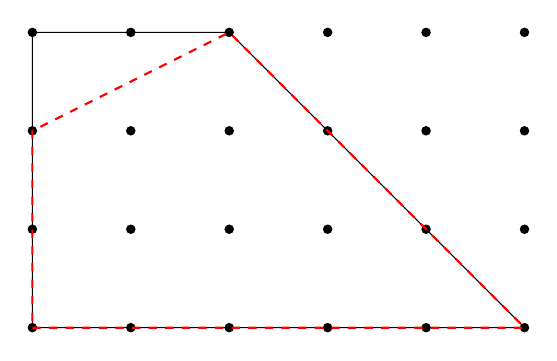
\begin{tikzpicture}

\foreach \x in {0,1,2,3,4,5}
   \foreach \y in {0,1,2,3} 
      \draw[fill] (5/4*\x,5/4*\y) circle (1.5pt) coordinate (m-\x-\y);

% using named coordinates
\draw (m-0-0) -- (m-5-0) -- (m-2-3) -- (m-0-3) -- cycle;
\draw[red, dashed, thick] (m-0-0) -- (m-5-0) -- (m-2-3) -- (m-0-2) -- cycle;

\end{tikzpicture}
\end{center}
\caption{The polygons $\Delta$ in black and $\Delta(f)$ in red for $f = x^5 + y^2 + x^2 y^3 + 1$ in example of Proposition \ref{example_weak_only}.}
\end{figure}
\end{prop}

\begin{proof}
See [Castrk]. The proof uses the theory of trigonal curves and the canonical embedding using that $\Delta^{(1)}$ and $\Delta$ have the same normal fan in this case. (GIVE MORE DETAILS). We can understand intuitively why this example works. The toric variety $\Toric_{\Delta}$ is a Hirzebruch surface and the curve $C_0^\Delta \embed \Toric_{\Delta}$ is tangent to the torus divisor at the component defined by the vertex $V = (0,3)$ in the polygon $\Delta$ showing that this curve is not $\Delta$-nondegenerate. Furthermore, the Hirzebruch surface has a single parameter family of automorphisms which translates the tangency point along the toric divisor which is why no equation for $C_0$ can be $\Delta$-nondegenerate. Notice that $\Delta(f) \subsetneq \Delta$ and the normal fan of $\Delta(f)$ contains an additional ray. Therefore, $\Toric_{\Delta(f)}$ corresponds to the toric blowup of the tangency point which turns the tangency into a transverse intersection which explains why $f$ is $\Delta(f)$-nondegenerate which is easily verified by a computation of the derivatives.
\end{proof}

\begin{figure}
\begin{center}
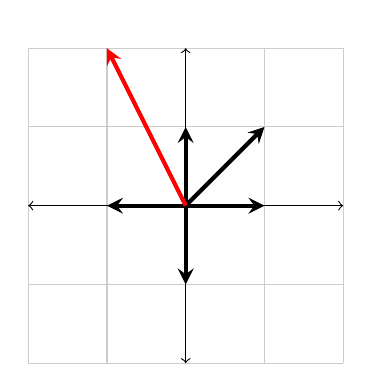
\begin{tikzpicture}
  \draw[thin,gray!40] (-2,-2) grid (2,2);
  \draw[<->] (-2,0)--(2,0) node[right]{};
  \draw[<->] (0,-2)--(0,2) node[above]{};
  \draw[line width=1.5pt,-stealth](0,0)--(1,1) node[anchor=south west]{$ $};
  \draw[line width=1.5pt,-stealth](0,0)--(1,0) node[anchor=south west]{$ $};
  \draw[line width=1.5pt,-stealth](0,0)--(0,1) node[anchor=south west]{$ $};
  \draw[line width=1.5pt,-stealth](0,0)--(0,-1) node[anchor=north east]{$ $};
  \draw[line width=1.5pt,-stealth](0,0)--(-1,0) node[anchor=south west]{$ $};
  \draw[line width=1.5pt,red,-stealth](0,0)--(-1,2) node[anchor=south west]{$ $};
\end{tikzpicture}
\end{center}
\caption{Rays of the normal fans of $\Delta$ (black) and $\Delta(f)$ (red). Notice that the normal fan of $\Delta(f)$ gives a toric blowup of the fan of $\Delta$.}
\end{figure}

\subsection{Generic Curves Do Not Live on Toric Surfaces (WIP)}

\begin{lemma}
Let $C$ be a curve over $k$. Then $C \times_k \P^1_k$ is unirational iff $C \cong \P^1_k$.
\end{lemma}

\begin{proof}
Suppose there is a dominant rational map $\P^2_k \rat C \times_k \P^1_k$. 
\end{proof}

\begin{theorem}[Harris-Mumford]
Generic curve .... 
\end{theorem}

\begin{theorem}
A generic curve (DEFINE!) of genus $g \ge 23$ cannot embedd into any (SMOOTH?) toric surface. 
\end{theorem}

\begin{proof}
Given an embedding $C \embed X$ into some toric surface $X$ we get $\T^2 \times_k C \embed \T^2  \times_k X \to X$ giving a family of curves in $X$. (WHAT HAPPENS IF THIS FAMILY IS TRIVIAL? I.E. FIXED POINTS OF TORUS ACTION.) 
This implies that $H^1(X, \struct{X}(C)) \ge 2$ (USE PICARD VARIETY ARGUMENT). Therefore, we may apply the Harris-Mumford (CITE) theorem to conclude that $X$ is birational to $C \times_k \P^1_k$ for the general curve $C$. However, since $X$ is toric, this implies that $C \cong \P^1_k$ but we have assumed that $g > 0$. 
\end{proof}

\subsection{Curves in Hurzburch Surfaces (DO!)}

(WORK ON THIS)
